\chapter{Introduction}\label{sec:intro}
Theoretically, fuel efficiency increases concomitantly with increasing turbine inlet temperature, but the lack of suitable materials with higher temperature capabilities (Figure~\ref{fig:TET}) has resulted in diminishing returns in fuel burn over the last 30 years (Figure~\ref{fig:FuelBurn}). Additionally, Dimiduk and Perepezko have recently shown that, on the contrary, over the last 70 years, marginal jet engine fuel efficiency has in fact decreased with rising turbine inlet temperatures ~\cite{dimiduk03} due to the energy required to operate the intricate cooling systems required by the 2$^{nd}$ and 3$^{rd}$ generation nickel-base superalloys used in the hot sections of commercial jet engines.  Using alternative materials that do not require cooling at current operating temperatures will result in improvements in engine efficiency.
%
\begin{figure}[htbp]
\begin{center}
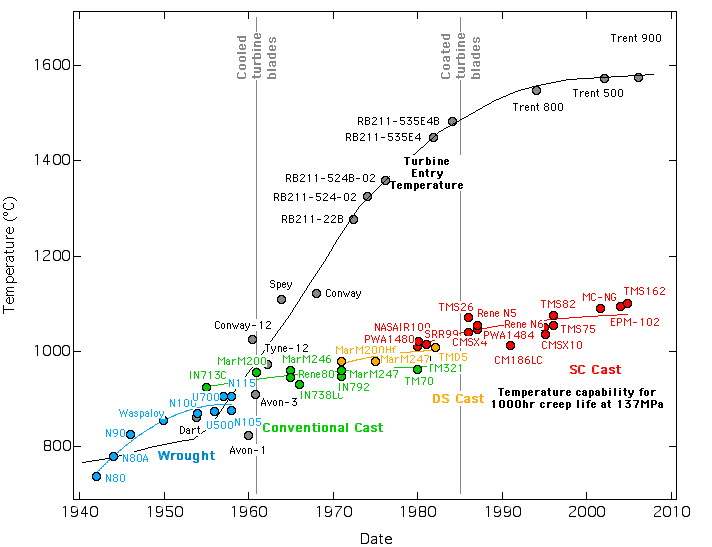
\includegraphics[width=\textwidth]{TET}
\caption{Evolution of the turbine entry temperature (TET) capability of Roll-Royce's civil aeroengines, from 1940 to present.}\label{fig:TET}
\end{center}
\end{figure}
%
\begin{figure}[htbp]
\begin{center}
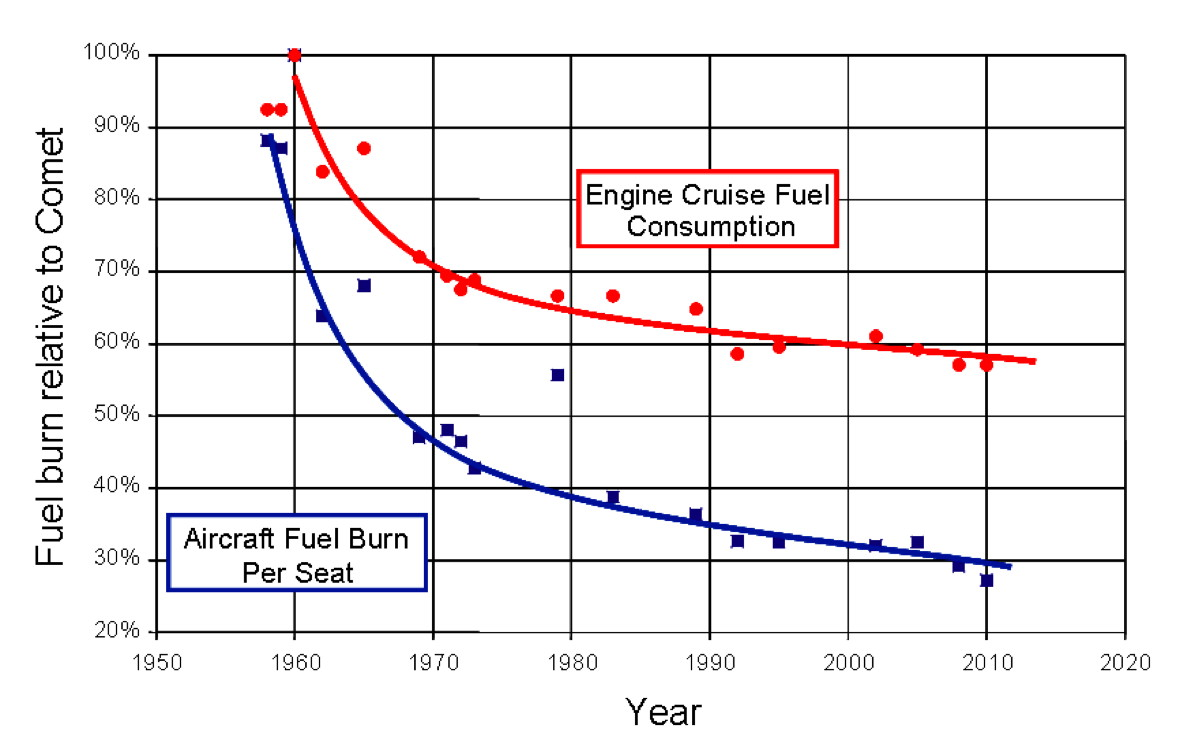
\includegraphics{FuelBurn}
\caption{Fuel burn of Rolls-Royce's civil jet engines, relative to the Comet, from 1960 to present. (Data courtesy of Rolls-Royce masterclass)}\label{fig:FuelBurn}
\end{center}
\end{figure}
%

We want to understand the issues to be faced when designing materials to supercede the commercial nickel-base superalloys used currently. Superalloys have enjoyed unparalleled success for the last 80 years as the high temperature load-bearing material to use ~\cite{reed06}, and there are solid reasons for this. They have a high homologous temperatures, are very resistant to mechanical degradation at high operating temperatures, possess excellent environmental resistance, and are robust, tough and easily machinable ~\cite{betteridge87, sims87}. Knowing how superalloys have evolved, and understanding the difficulties encountered and the successes celebrated thus far by the nickel-base superalloy community provides the starting point for this thesis. An investigation of the most advanced 4$^{th}$ generation superalloys forms the first part of this thesis; the second part is an examination of potential replacement systems and some preliminary results from these materials. 

The incremental approach taken has been to design superalloys with higher temperature capabilities ~\cite{reed06, cumpsty97}.   There have been 3 recognised generations of superalloys defined by alloy composition range. The latest 4$^{th}$ generation superalloys are distinguished by the presences of ruthenium.  Ruthenium was found to suppress topologically close-packed (TCP) phase precipitatation very effectively with little observable detriment to the other desirable properties of superalloys ~\cite{yeh04}.  This permitted the concentration of rhenium, a powerful solid solution strengthener, to be almost doubled without substantial reductions in microstructural stability.  These advanced superalloys with high refractory contents have more highly negative lattice misfits than earlier superalloys, and would directionally coarsen more easily upon the presence of applied stress.  These coarsened precipitates, also known as rafts, are beneficial against high temperature creep.  However, it turns out that this early stage ``rafting" invariably compromises intermediate temperature creep properties, allowing dislocations to cut through them more easily than through unrafted finer cubiodal precipitates ~\cite{hobbs08}.  Understanding the factors that induce early stage rafting, would enable us to determine how to effectively manage them.  

More radical alternative materials to superalloys include two broad classes of materials: intermetallics and ceramics. They offer substantial increases in temperature capability, but have many problems that have not been surmounted as of yet ~\cite{miracle94, kumar94, shah92, sauthoff88, kelly91, kelly96, jackson96, chang91, fleischer94, fleischer85a}. Most notably, their inherent low ductility and fracture toughness at room temperature cause them to have low impact tolerances and to be extremely difficult to process and machine. In this thesis, the compositions that have potential to offer a 100\celsius\ increase in temperature capability over current commercial superalloys will be listed. Systems of compositions that have the potential to realize room temperature fracture toughness and ductility that are higher than current intermetallics and ceramics, while providing the desired increase in temperature capability, will be identified. From literature, eutectic systems with a solid solution toughening phase and a silicide load-bearing phase demonstrate the capacity to fulfill the stated aims. These (Cr,V)$_{solid\ solution}$--(Cr,V)$_3$Si$_{intermetallic}$ eutectics will be characterised to understand their microstructural stability, failure mechanisms, high temperature creep mechanisms and oxidation character.
 
\chapter{Nickel-Base Superalloys}
\section{The Evolution of Nickel-Base Superalloys}

Sims' introduction of the origins of superalloy development in \emph{Superalloys II} ~\cite{sims87} and \emph{The Superalloys} by Reed ~\cite{reed06} both provide excellent overviews on this subject and should be consulted for more detail.  Figure~\ref{fig:evolution} beautifully sums up the evolution of nickel-base superalloys from conception in the 1930s to date, with strengthening phases shown in the top half, and the deleterious phases in the bottom half.
%
\begin{figure}[htbp]
\begin{center}
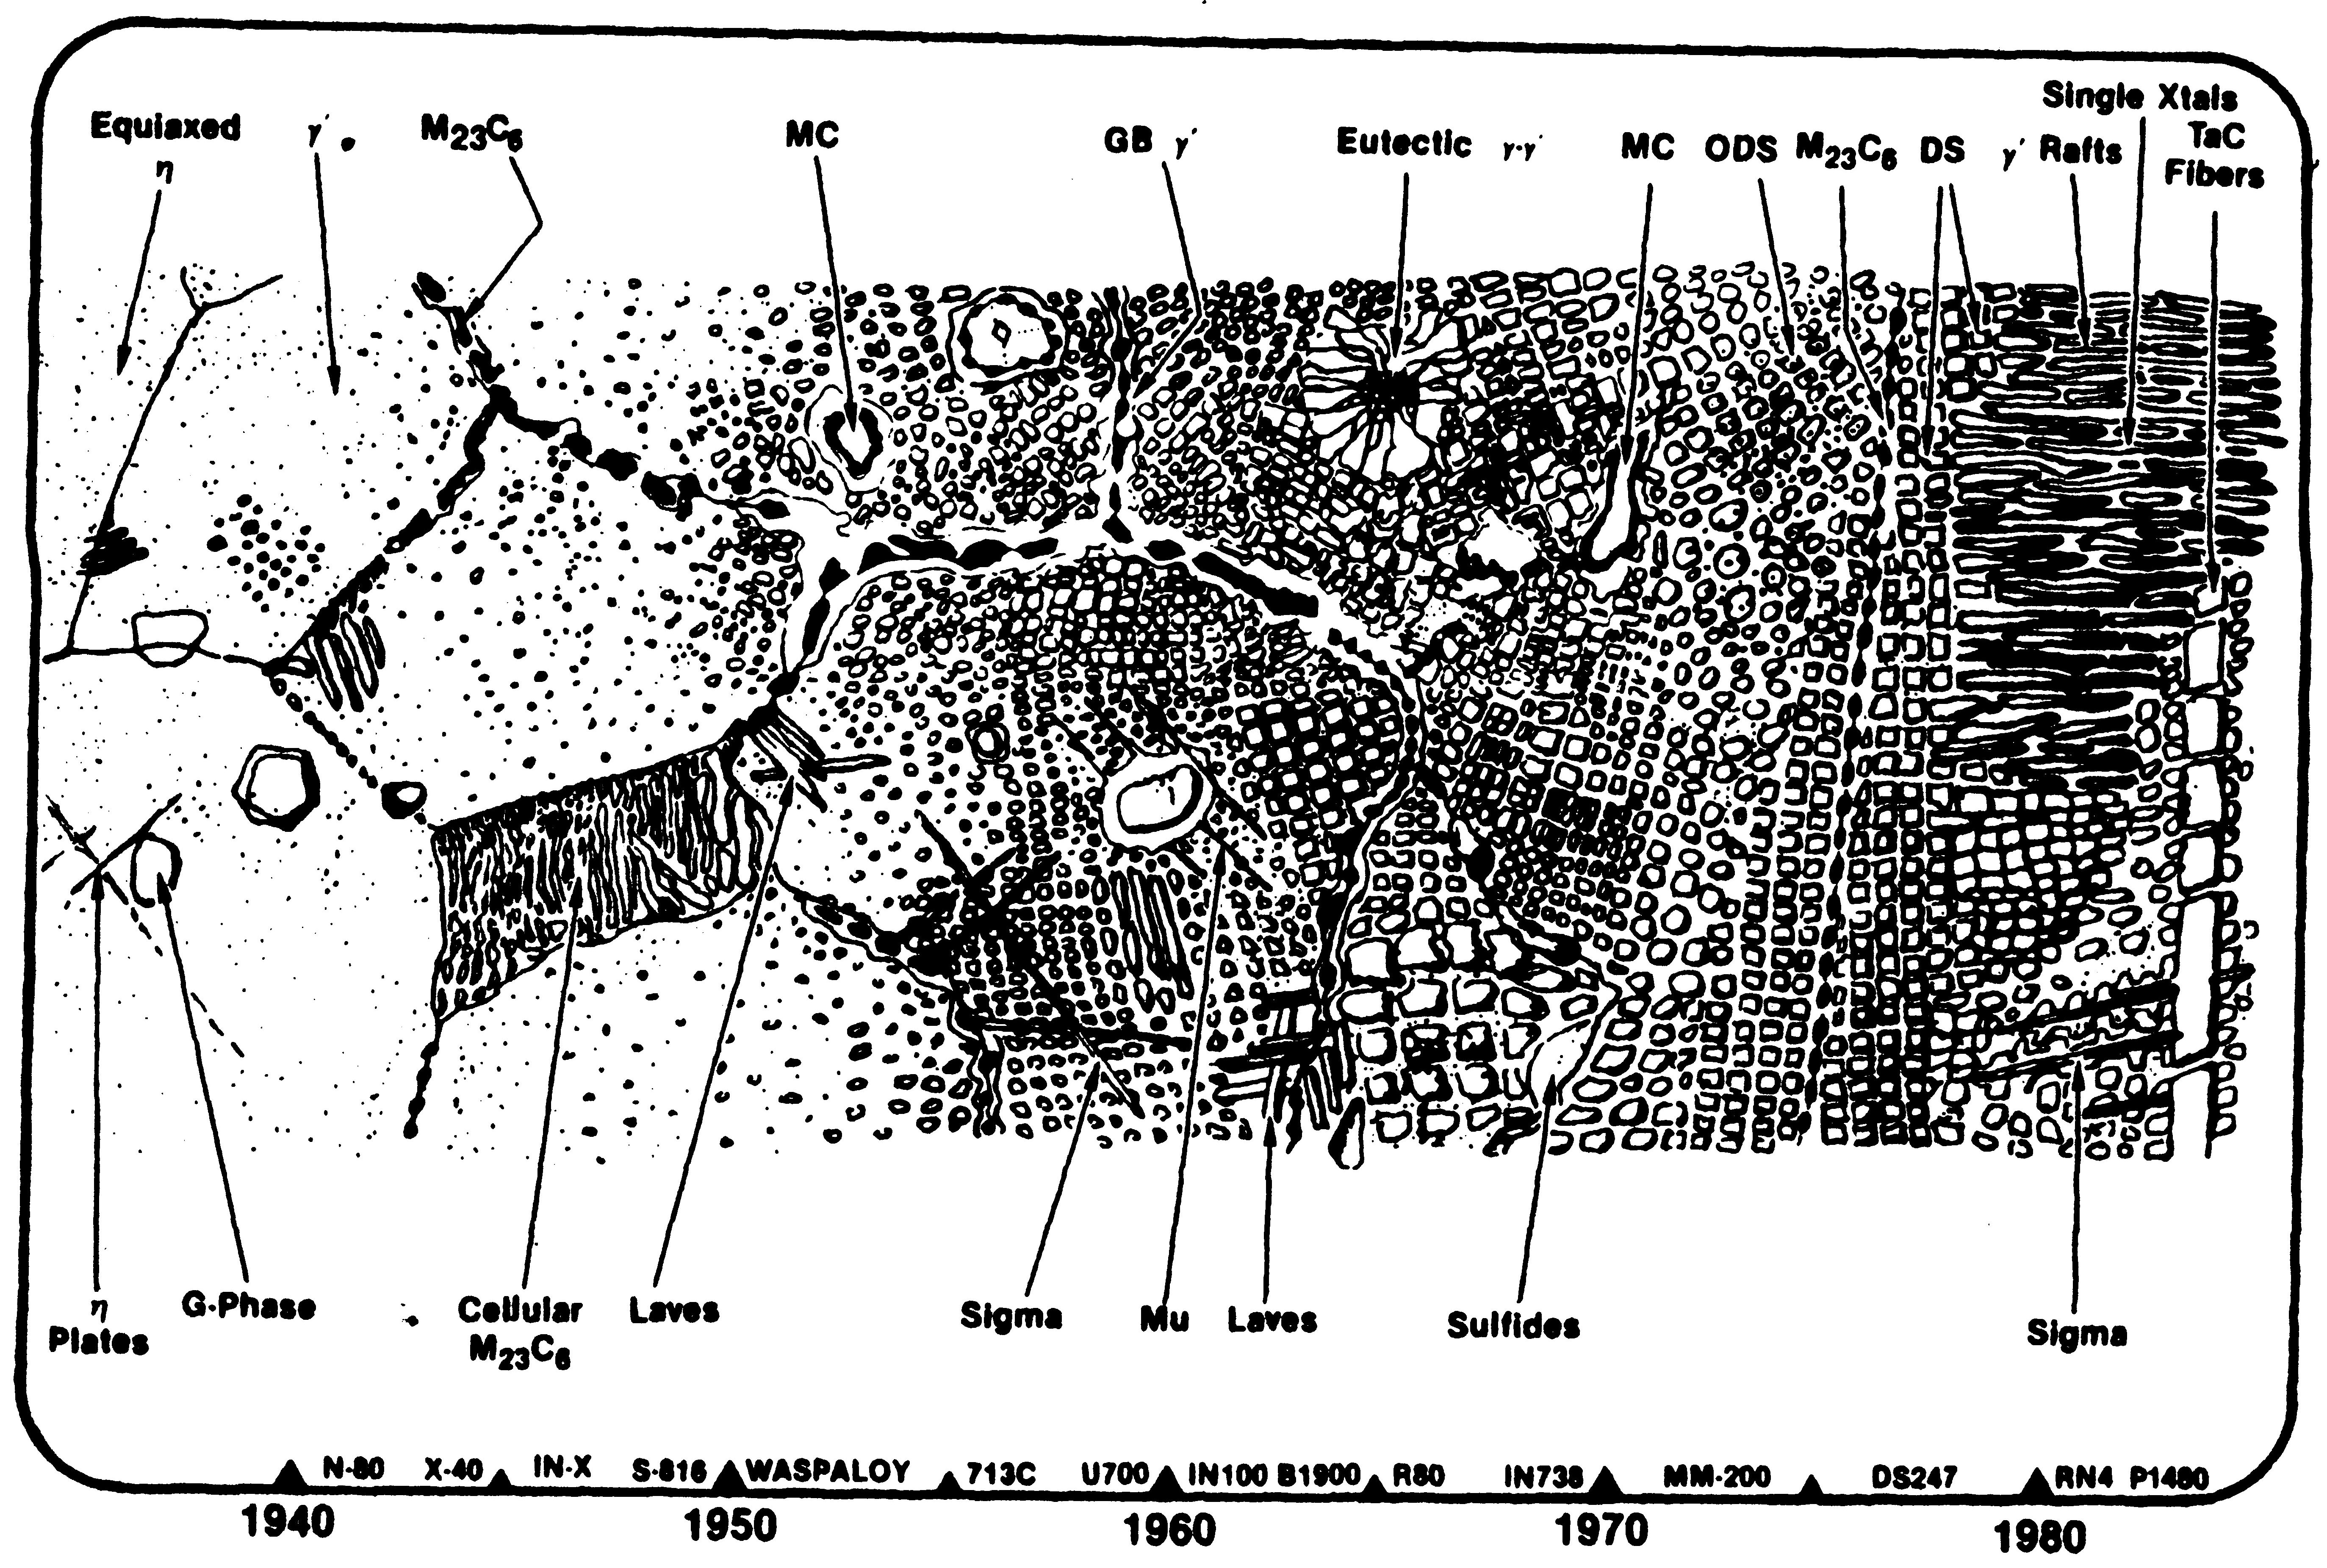
\includegraphics[height=5.5in, angle=90.6]{SuperalloyEvolution}
\caption{Evolution of blade material. Panorama of the development of nickel superalloy microstructure showing both useful and deleterious phases \cite{sims87}.}
\label{fig:evolution}
\end{center}
\end{figure}
%
Superalloys started out as a multi-grained FCC nickel-chromium austenite matrix, with carbides serving as the strengthening phase. This choice of having an FCC matrix is rather fortuitous, as it is now known to be the atomic configuration that can best maintain strength to high homologous temperatures. Aluminium was then found to effectively improve high temperature oxidation resistance, due to the transition of oxide structure from chromia to alumina. Moreover, unbeknownst to the metallurgists, their additions of aluminium also created a small volume fraction of coherent Ni$_3$Al $\gamma'$ precipitates, the sole strengthening phase employed in the most advanced single crystal nickel-base superalloys today. 

With the advent of electron microscopy a decade later, metallurgists were then able to identify carbides and $\gamma'$, and quantify their effects on the high temperature mechanical behaviour alloys. This led to alloys being designed with increasing volume fractions of both phases.  Refractory elements were then found to impart strength to both the solid solution and the precipitates.  Molybdenum was added, followed by tantalum and tungsten. This compromised microstructural stability, and precipitated the formation of embrittling TCP phases. These TCP phases serve as crack nucleation sites, inducing creep cavitation ~\cite{reed99} and causing pre-mature creep failure at high temperatures ~\cite{yeh04}.  As these phases consist mostly of refractory elements, surrounding regions get depleted of their strengthening elements, and this exacerbates localized pre-mature failure. The threshold for solid solution strengthening had been reached.  

Directional solidification was then introduced, allowing for crystal alignment and orientation.  Single crystal superalloys were made possible with the application of grain selectors, which made carbides obsolete, as they were no longer necessary as grain boundary strengtheners.  This widened the heat treatment window and allowed for more complete heat treatment of superalloys.  

In 1986, rhenium was discovered to effectively improve the high temperature mechanical properties of superalloys via solid solution strengthening of the matrix.  Its low diffusivities in nickel at high temperatures were also found to interfere with diffusional creep mechanisms that occur at high temperatures.  Regrettably, its addition induced microstructural instability and inhomogeneity; 2 at.\% resulted in sufficient TCP precipitation to cause premature creep rupture. The alloying ceiling had been reached again.  

Ruthenium was subsequently found to reduce this propensity for TCP formation, by allowing superalloys to tolerate a higher rhenium content. The crystal lattice has to undergo further distortion to accommodate these large refractory atoms, resulting in a more negative lattice misfit.  These superalloys suffer from premature creep failure at intermediate temperatures of 950\celsius, but the reasons for this have not been determined.

Although much of superalloy development has been empirical, the superalloy community is developing advanced modelling techniques to expediate the alloy development process.  Non-linear regression analyses and phase diagram simulations are being used in the prediction of material properties and microstructure. Finite element modelling is used in optimisation of solidification processes.  However, composition, microstructure and processing are very much interdependent. Therefore, it is essential to couple models to incorporate all aspects of alloy design when designing a bespoke product with specific properties.

This is where the superalloys community stands at currently.

\section{Microstructure and Deformation}

In order to understand the consequences of rafting at intermediate temperatures and intermediate stress, it is necessary to detail the superalloy microstructure and its deformation mechanisms during creep in this regime.

\subsection{Dislocations}

The $\gamma$ phase is a nickel-base solid solution with a disordered fcc lattice. The $\gamma'$ intermetallic phase is a Ni$_3$Al fcc superlattice with the L1$_2$ structure. There is a coherent cube-cube orientation  relationship between $\gamma$ and $\gamma'$, and coherent $\gamma'$ precipitates form when lattice misfit is small. These precipitates serve as barriers to dislocation motion, hardening the material ~\cite{copley67}. 

For dislocation motion to proceed, precipitate circumvention or cutting must occur. In commercial blade superalloys, looping of dislocations around precipitates is made difficult by having a high volume fraction of small, discrete particles \cite{reed06, copley67}. This results in narrow matrix channels, which increase the Orowan stress. Dislocation climb is limited by the diffusion rate of the elements at and around the dislocation, and its rate increases with temperature.  During precipitate cutting, an $\frac{a}{2}\left<110\right>$ matrix dislocation moving through an ordered superlattice forms an anti-phase boundary (APB).  The high energy associated with these APBs inhibit dislocation motion through the ordered precipitate.  To minimise this formation energy, the $\frac{a}{2}\left<110\right>$ dislocations typically accomplish precipitate cutting by travelling in pairs or in groups.  The distance between a dislocation pair is dictated by the formation energy of the APB between the dislocations in the precipitate, 
their elastic repulsion energy, the temperature and magnitude of the applied stress. When conditions are unfavourable for either mechanism to proceed, dislocation pile-up occurs at the matrix-precipitate interface, hardening the material.

%There is a driving force from elastic energy of dislocation strain fields for each superdislocation to dissociate into two $\frac{a}{2}\left<110\right>$ dislocations separated by an APB on the $\{111\}$ plane. 

As temperature rises up to 800\celsius, dislocations cross-slip so that the APB fault lies on the $\{001\}$ plane where it has a lower energy. The dislocations become sessile, forming Kear-Wilsdorf locks ~\cite{reed06}. These locks are the cause of the yield stress anomaly, where yield strength increases with temperature. Above 800\celsius, $\gamma'$ softening occurs because the threshold stress for unlocking becomes lower.

MacKay and Ebert hypothesized that the misfit dislocations in the $\gamma$/$\gamma'$  interface are present to relieve the interfacial strains arising from the large negative mismatch~\cite{mackay83}.  These dislocations are similar to those observed in the initial stages of coherency loss of the $\gamma'$ precipitate in long-time aged superalloys, having three-dimensional octagonal networks of $\frac{a}{2}\left<110\right>$ edge dislocations.  Misfit dislocations relax the internal strain energy of a material due to large misfit, therefore decreasing the internal energy of the system. 

Harada and coworkers are of the opinion that dislocations form networks in the $\gamma$ channels that serve as a barrier to precipitate shear, and that these networks hinder the dislocations from entering the vertical $\gamma$ channels.  They hypothesize that superalloys with denser networks would be more resistant to high temperature creep ~\cite{harada06}.

As creep resistance is inversely related to the rate of dislocation motion, an effective means of hindering dislocation motion is precipitate volume fraction optimisation.  The optimal $\gamma'$ volume fraction would minimise the widths of the matrix channels between the precipitates whilst maintaining discreet precipitates.  Dislocations must bow more to enter the matrix channels, which requires higher stress.  Refractory element additions are beneficial as they lower diffusion coefficients and their larger diameters strengthen the solid solution, providing resistance to dislocation motion.


\subsection{Lattice Misfit}

As discussed previously, it is generally desirable for alloys to contain significant quantities of refractory elements to improve creep performance.  Of these elements, only tungsten displays limited partitioning between the matrix and precipitates. Molybdenum and rhenium partition preferentially to the matrix, whilst tantalum partitions to the precipitates \cite{reed04}. In general, however, higher concentrations of refractory elements are typically in the matrix than in the precipitates. The matrix thus has a larger coefficient of thermal expansion than the precipitates. As a consequence, the lattice misfit is typically observed to become more negative upon heating. This has a profound impact on the magnitude of the misfit seen in the alloy at elevated temperature depending upon the composition and hence also the room temperature misfit.

Lattice misfit quantifies the extent of coherency, with larger values signifying higher coherency strains, where the lattice parameter of the precipitate is substantially larger than that of the matrix, or vice-versa.  The lattice misfit is defined by \cite{nabarro96}:
%
\begin{equation}
\delta = \frac{2(a_{\gamma'} - a_\gamma)}{a_{\gamma'} + a_\gamma}
\label{eq:misfit}
\end{equation}
%
The mechanical properties of superalloys have been found to be heavily dependent on $\gamma$/$\gamma'$ interfacial coherency ~\cite{reed06}.  Dislocation movement is impeded by a high lattice misfit due to an increase in elastic strain in the slip plane.  For alloys with positive misfits at room temperature the misfits decrease in magnitude upon heating and may become negative.  In contrast, for an alloy with a negative misfit under ambient conditions, the magnitude of the misfit will typically increase monotonically upon heating.  

With high misfit values, the interfacial energy increases, leading to a more rapid loss of coherency and an increase in the rate of precipitate coarsening.  With the discovery that ruthenium addition allows for increased refractory solubility, refractory element contents have increased, and misfit values have risen accordingly.  It is clear that these higher misfits will not allow coherency to be maintained at the precipitate-matrix interface.  Loss of coherency between the matrix and the precipitate, either by thermal relaxation or through the accumulation of dislocation debris following mechanical deformation, may lead to a reduction in the mechanical properties of the alloy.

\subsection{Creep}

Creep is the plastic deformation at stresses below the flow stress and is dependent on stress, time and temperature ~\cite{nabarro96}.  Reed states that Ni-based single crystal superalloys undergo three stages creep deformation: primary, secondary and tertiary.  He identifies three regimes of creep: primary, tertiary and rafting \cite{reed99}.  

In this report, comments are restricted to the intermediate temperature/intermediate stress tertiary creep regime, with temperature between 850--1000\celsius, and stress between 300--500 \mega\pascal.  In this regime, the three stages of creep are not distinct; instead, there is minimal primary creep, and creep appears to increase logarithmically with time, as the creep strain rate is proportional to the accumulated macroscopic creep strain.

The relevant regime of creep plasticity for the intermediate stress/intermediate temperature creep condition of single crystal nickel-base superalloys is power law creep.  It essentially describes deformation produced by the glide of dislocations in the $\gamma$ phase.  This deformation is limited by dislocation climb around coherent $\gamma'$, which effectively serve as obstacles to prevent plastic flow.  Thermally activated diffusion allow dislocations to climb out of the slip plane, over $\gamma'$ precipitates, and continue to glide along another.  The creep rate is determined by dislocation density and the rate of dislocation movement, and is described by the Orowan equation \cite{nabarro95}:
%
\begin{equation}
\dot{\gamma}  = \rho  b  v  
\end{equation}
%
During high temperature creep, precipitate cutting is difficult due to the lower stress conditions experienced, and this results in dislocations being trapped within the $\gamma$ matrix channels, making dislocation climb around the $\gamma'$ precipitates the dominant mechanism (Figure \ref{fig:LDSX8disloc}). Under intermediate temperature/intermediate stress creep conditions, some precipitate cutting occurs, but precipitate circumvention is dominant. Under low temperature/high stress creep, the stress is experienced by the alloy is high enough to allow precipitate cutting as the principal mechanism for dislocation motion(Figure \ref{fig:LDSX1faults}).
%
\vspace{1cm}
\begin{figure}[H]
\begin{center}
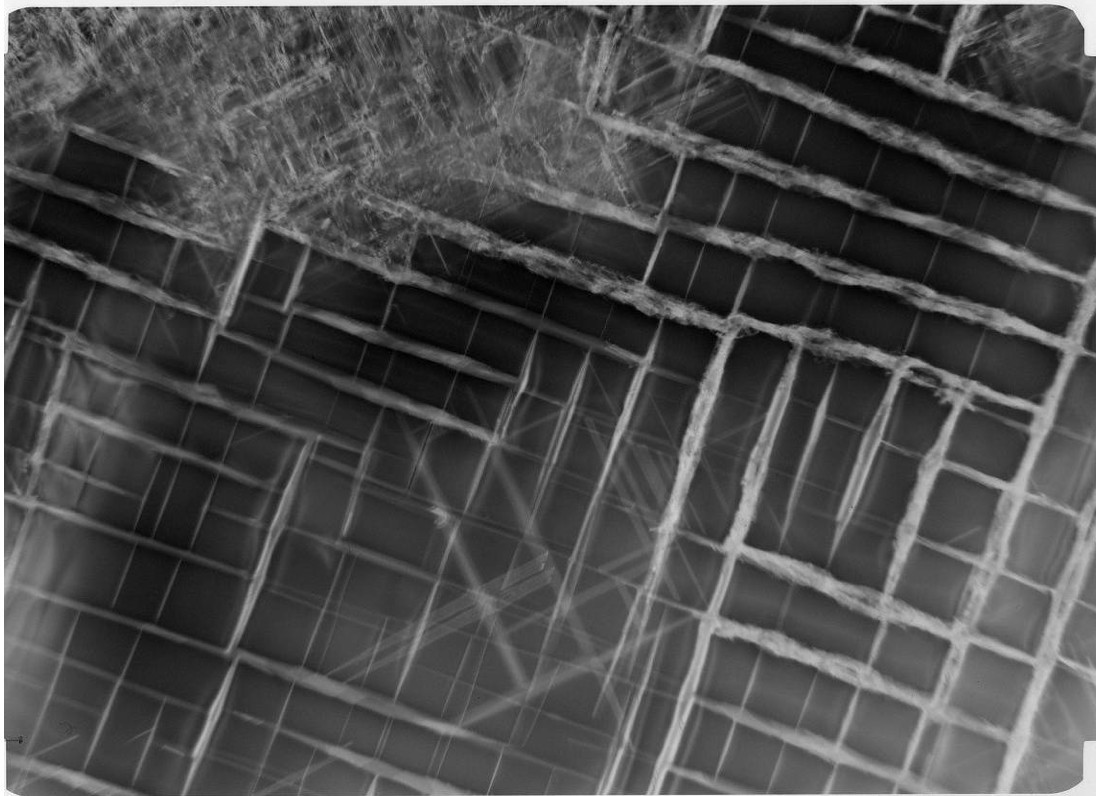
\includegraphics{LDSX8disloc}
\caption{Dislocations located mostly in the $\gamma$ channels of LDSX--8 after heat treatment; very few dislocations have entered the $\gamma'$ precipitates. (courtesy of H.T. Pang)}\label{fig:LDSX8disloc}
\end{center}
\end{figure}
%

\begin{figure}[H]
\begin{center}
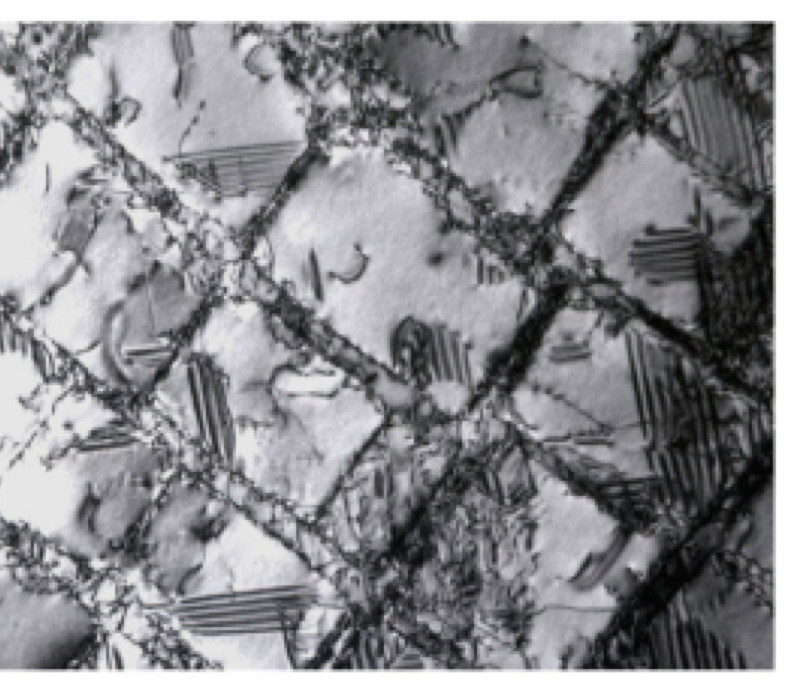
\includegraphics[width=8cm]{LDSX1faults}
\caption{Stacking faults in $\gamma'$ precipitates formed due to dislocation cutting in LDSX--1 after low temperature creep at 750\celsius/800\mega\pascal. (courtesy of L.J. Zhang)}\label{fig:LDSX1faults}
\end{center}
\end{figure}
%
\subsection{Rafting}
When a negatively misfitting alloy is subject to tensile stress at elevated temperatures of above 900\celsius, dislocations form and accumulate in the horizontal channels, relieving the misfit stresses and allowing for the relaxation of coherency stresses on the horizontal $\gamma$/$\gamma'$ interfaces (Figure \ref{fig:CoherencyStress}). This coincides with the cuboidal as-aged $\gamma'$ precipitates coalescing into rafts normal to the tensile loading axis.  This process is known as rafting.  When extensive rafting occurs, the encapsulating $\gamma$ matrix will no longer remain interconnected(Figure \ref{fig:LDSX6rafts}).  
%
\begin{figure}[H]
\begin{center}
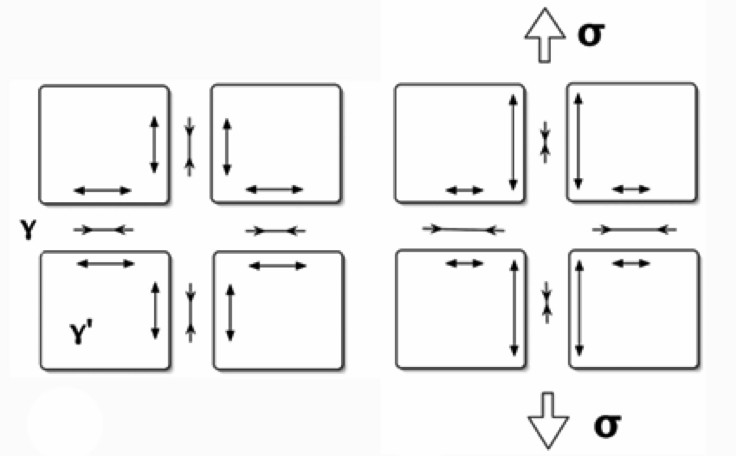
\includegraphics[width=10cm]{CoherencyStress}
\caption{Schematic of coherency stresses arising from an applied tensile stress. (adapted from \cite{reed06})}
\label{fig:CoherencyStress}
\end{center}
\end{figure}
%
\begin{figure}[H]
\begin{center}
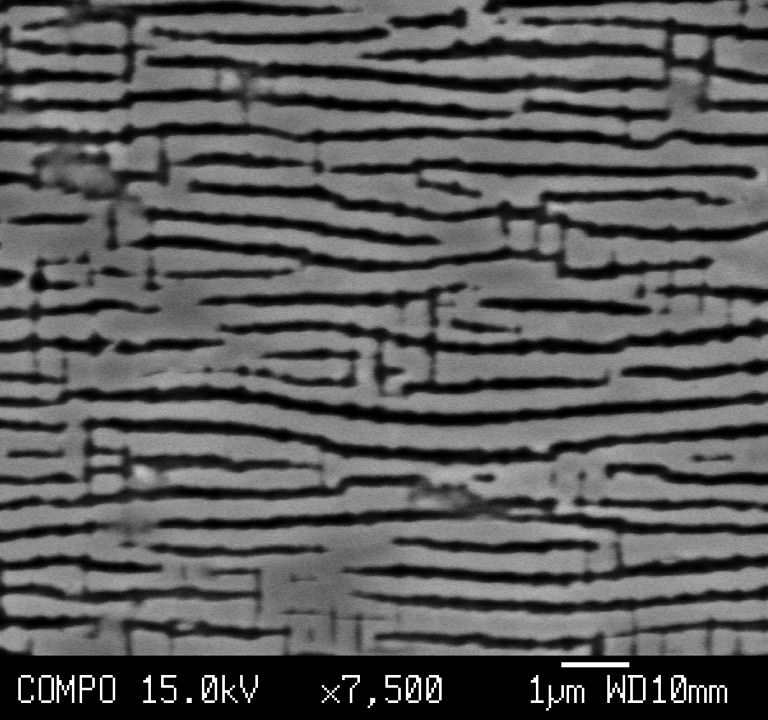
\includegraphics{LDSX6rafts}
\caption{Rafted microstructure of LDSX--6 interrupted after primary creep and subsequent thermal exposure for 500 hours at 950\celsius.}
\label{fig:LDSX6rafts}
\end{center}
\end{figure}
\vspace{-1cm}
%
In the early 1980s, rafting was believed to weaken the alloy's creep properties, due to the increase in interlamellar spacing.  Larger inter-lamellar spacing translates to larger $\gamma$ channels, which do not hinder dislocation motion.  This led to the development of alloys with lower lattice misfit, to obtain minimum coarsening rates with the intention of maximizing creep resistance.  MacKay and Ebert then reported that directional coarsening in single-crystal superalloys with large negative misfit increased creep life by 4 times in the $\left<100\right>$ orientation at 982\celsius\ \cite{mackay83}.  They found rafts were effective barriers to dislocation climb around $\gamma'$.

They observed that once rafts were formed during steady-state creep, the lamellae stabilise and do not undergo further rafting.  A limit had been reached where substantially higher amounts of total strain was required to induce further rafting.  From this, they hypothesised that rafting may be a strain-controlled and time dependent phenomenon.

Factors influencing rafting kinetics are still a subject of controversy.  Reed et al. agree with MacKay's observation that the rafted structure is largely completed at the very early stages of deformation.  Since the rafts are established early, the dislocations, being unable to cut through them under the high temperature/low stress creep conditions, can only move via precipitate circumvention.  The plate-like morphology of these rafts makes circumvention very difficult.  This is probably why superalloys with rafted microstructure perform well during high temperature creep.

Although rafts are beneficial for high temperature creep, they have been found to be detrimental for creep at lower temperatures ~\cite{hobbs08}.  Blade alloys are subject to higher stresses at lower temperatures, this enables dislocations to cut through precipitates.  Since as heat-treated, uncoarsened cuboidal precipitates are finer than the ``rafts", dislocations have a larger energy barrier to surmount for precipitate cutting.  Also, they have a smaller average interparticle spacing, which impedes Orowan dislocation bowing, as the dislocation radius must be very large in order to have sufficient energy to force their way into the smaller $\gamma$ channels.


\section{Background to Experimental Work}
\subsection{The Kinetics of Rafting}

The thermodynamic driving force for rafting depends on the lattice misfit and applied stress.  V\'{e}ron et al. noticed that strain induced during creep seems to be responsible for the rafting phenomenon, and postulated that there is a critical density of plasticity-induced dislocations necessary to induce rafting, and that additional dislocation density above this threshold would have no influence on rafting \cite{veron96}.

A novel method was used by Matan et al. to precisely quantify the kinetics of rafting in a commercial 2$^{nd}$ generation superalloy, CMSX 4, with the aim to evaluate the influence of rafting on creep deformation \cite{matan99}.  Interrupted creep tests at 950\celsius/185 \mega\pascal\ were performed on single crystal heat-treated creep specimens with $\left<100\right>$ orientation parallel to the applied stress, using 20 kN constant load creep testing machines.  The tests were interrupted  at 150, 280, 500, 695, 1060 and 1170 hours.  The tested specimens were sectioned axial to the direction of applied stress, and micrographs were taken and stereologically characterised.  Degree of rafting was seen to increase with the length of creep testing.

The threshold strain for rafting to proceed in the absence of applied stress was determined.  The threshold strain was found to be 0.10$\pm$0.03\%.  When a specimen was strained beyond the threshold strain, it continues to raft during subsequent annealing in the absence of applied stress.  If accumulated strain is below the threshold strain, subsequent annealing does not promote further raftingMatan et al. postulated that the thermodynamic driving force and the kinetics of rafting in the plastic regime would be correlated to the lattice misfit. This will be investigated by looking at three alloys in the LDSX series with representative low, medium and high lattice misfits.

\subsection{Effect of Misfit on Creep Properties}

The LDSX series comprises of eight 4$^{th}$ generation alloys that has been developed at the Rolls-Royce University Technology Centre are currently undergoing evaluation.  The nominal compositions and predicted misfit values by JMatPro$^{\copyright}$ are shown in Table~\ref{tab:LDSXcomps}.

Alloys with representative low, intermediate and high misfits, LDSX--1, 6 and 8, have been chosen for this study, as seen in Figure \ref{fig:MisfitJMatPro}.  LDSX--1 is the least alloyed, with the lowest content of Mo, Re and W, and consequently, possesses the lowest misfit.  LDSX--8 has the highest refractory element content, and the highest predicted misfit.  A commerical second generation superalloy, CMSX-4, will be used as reference.
%
\begin{table}[htdp]
\begin{center}
\begin{tabular}{lccccccccccc}
\hline\hline
Alloy 	&     Ni    &  Al   &  Co  &   Cr &   Mo     &Ti     & Ta    & W     &Re &    Ru    & Hf\\\hline
LDSX-1  &   Bal.&    6.0&    3.0&     3.0&     2.5&    0.25&    6.5&    2.9&    6.2&     3.5&     0.1\\LDSX-2    & Bal.&    6.0&    8.0&     3.0&     5.0&    0.25&    6.5&    2.9&    6.2&     3.5&     0.1\\LDSX-3     &Bal.&    6.0&    3.0&     3.0&     5.0&    0.25&    6.5&    4.8&    6.2&     3.5&     0.1\\LDSX-4 &    Bal.&    6.0&    8.0&     3.0&     2.5&    0.25&    6.5&    4.8&    6.2&     3.5&     0.1\\LDSX-5 &    Bal.&    6.0&    8.0&     3.0&     2.5&    0.25&    6.5&    2.9&    6.2&     5.0&     0.1\\LDSX-6  &   Bal.&    6.0&    3.0&     3.0&     2.5&    0.25&    6.5&    4.8&    6.2&     5.0&     0.1\\LDSX-7  &   Bal.&    6.0&    3.0&     3.0&     5.0&    0.25&    6.5&    2.9&    6.2&     5.0&     0.1\\LDSX-8  &   Bal.&    6.0&    8.0&     3.0&     5.0&    0.25&    6.5&    4.8&    6.2&     5.0&     0.1\\
\hline\hline
\end{tabular}
\end{center}
\caption{Nominal compositions of LDSX--1 to 8.}\label{tab:LDSXcomps}
\end{table}
%
\begin{figure}[H]
\begin{center}
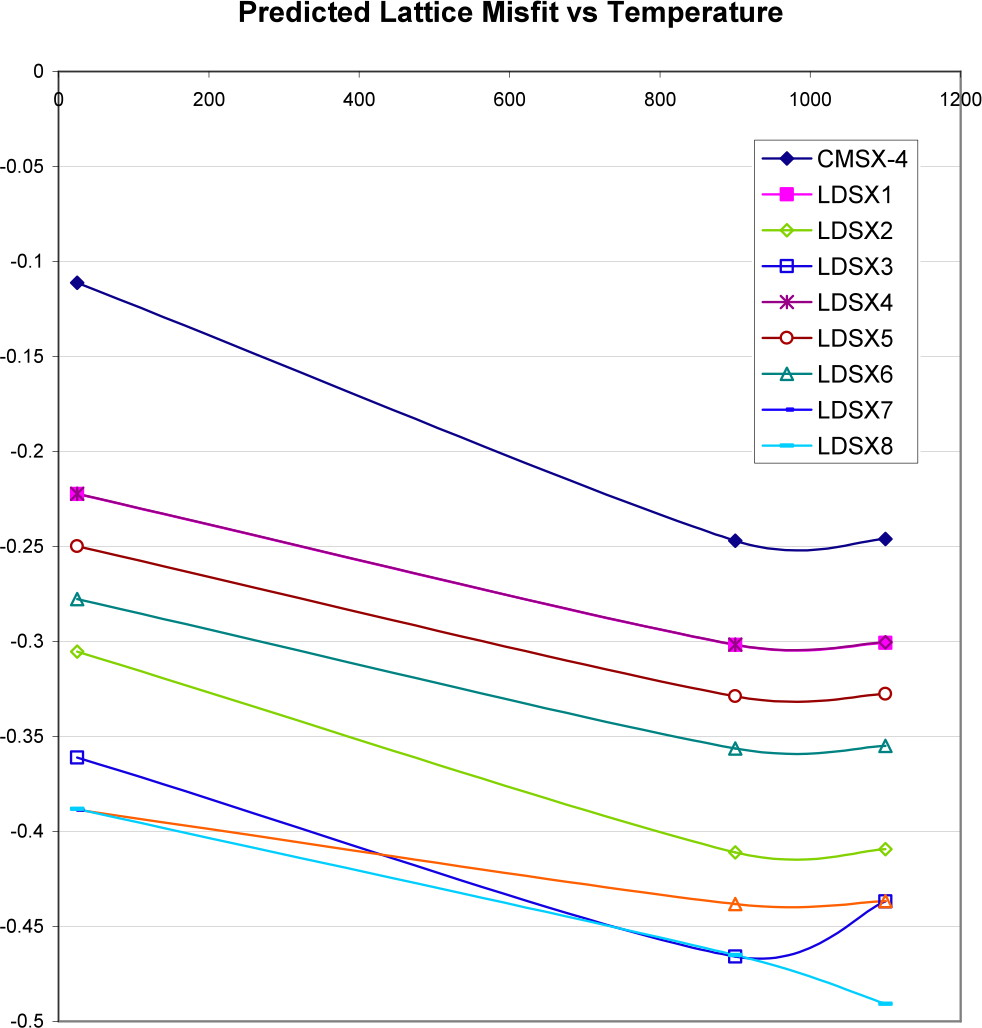
\includegraphics{MisfitJMatPro}
\caption{Predicted misfit as a function of temperature for LDSX--1, 6 and 8.}
\label{fig:MisfitJMatPro}
\end{center}
\end{figure}
%
The more heavily alloyed LDSX--6 with higher lattice misfit took a longer time than LDSX--1 to reach the same elongation.  The most heavily alloyed LDSX--8, suffered from premature rupture, and had half the rupture life of LDSX--1.  Additionally, LDSX--8 had no visible incubation period, and a mere two hours of primary creep.  This premature failure can be due to several factors.  It has a highly negative misfit, and is noted to be prone to TCP precipitation. 




\section{Experimental Work}

Bars of alloys designated LDSX--1, 6 and 8 were directionally-solidified to produce single crystals with $\left<001\right>$ orientation at the Precision Casting Facility (PCF) in Derby, England.  The bars were solution treated to eliminate casting segregation: LDSX--1 at 1340\celsius\ for 10 hours, LDSX--6 at 1340\celsius\ for 10 hours, and LDSX--8 at 1360\celsius\ for 15 hours.  They were then primary aged at 1150\celsius\ for 4 hours and secondary aged at 870\celsius\ for 16 hours to eliminate secondary $\gamma'$. 

Tensile creep specimens were machined from LDSX--1, 6 and 8.  Their $\theta$/$\rho$ angles, showing their relative orientation to the loading axis, were 4.2/36.4, 13.0/18.7 and 3.0/28.8, respectively.  They were crept at 950\celsius/375\mega\pascal\ and the tests were stopped when the onset of secondary creep was observable.  Sections were cut out from the gauge lengths of these interrupted creep specimens.  They were then subject to thermal exposure at 950\celsius, the temperature that the specimens were crept at, for a subsequent 10, 50, 100, 200, 500 or 3000 hours.  Microstructural examination was performed with a JEOL 6340F FEGSEM, where micrographs representative areas were taken to quantify microstructural stability and the extent of rafting in these alloys. 

Misfit measurements are difficult to obtain for nickel-base superalloys by diffraction using conventional laboratory X-ray sources.  The $\left<001\right>$ $\gamma$ peaks are invisible in fully ordered structures.  The $\left<001\right>$ $\gamma'$ peak is visible but it is very weak and requires a long data collection time when using a typical X-ray source available at universities.  This leads to instrumental line broadening, a source of error.  Also, the $\left<002\right>$ peaks of $\gamma$ and $\gamma'$ overlap and are very difficult to separate.  In order to split these peaks accurately, the $\left<001\right>$ $\gamma'$ peak position, which indicates its lattice parameter, can be used to ``fix" the position of the $\gamma'$ peak, which allows us to determine the peak position $\gamma$ through curve deconstruction. X-rays produced at a synchrotron are of higher intensity, and much shorter acquisition times would be required.  Measurements of the lattice parameters of the $\gamma$ matrix phases and $\gamma'$ precipitate phases of the alloys were performed on the BM28 beamline at the European Synchrotron Radiation Facility (ESRF) in Grenoble, France.  Monochromation of the X-rays was achieved by diffraction from a double-crystal Si $\{111\}$ monochromator to give an incident energy of 11.9 \kilo\electronvolt\ with a wavelength of 1.0418 \angstrom.  The beam was 0.5$\times$0.5 \milli\meter\ at full width at half maximum (FWHM), with a resolution of 1.7$\times$10$^{-4}$, and was focused on the sample surface using a torroidal mirror.

Transverse sections of the bars with $\left<001\right>$ nominally vertical were mounted on a goniometer head attached to an 11-axis Huber diffractometer.  This permitted the sample to be translated in x, y and z within the diffractometer and orientated in four circles ($\phi$ , $\chi$ , $\omega$, 2$\theta$).To establish the orientation of the sample, the 2$\theta$ angle was set at a value consistent with the expected lattice parameter of the material and $\phi$ varied until a strong diffraction signal was detected.  For samples with significant off-axis orientations, scans in $\phi$ were performed as chi was increased to locate the $\left(001\right)$ pole.  Once established, 2$\theta$ was increased to an angle consistent with diffraction from a $\left(111\right)$ pole and the sample reoriented accordingly before scanning in $\phi$ to indentify the pole.  Knowledge of the orientations of these two poles permitted automatic reorientation of the sample to other poles for detailed measurement.

The $\left(001\right)$ \& $\left(003\right)$ superlattice reflections and $\left(002\right)$ \& $\left(004\right)$ fundamental reflections were scanned in \emph{h} \& \emph{k} to generate two-dimensional reciprocal space maps.  It was considered necessary to characterise the superlattice reflections so that the lattice parameter of the $\gamma'$ could be uniquely determined and enable unambiguous identification of the contribution of the $\gamma'$ to the overlapping fundamental reflections.  The low atomic scattering contrast between the atoms occupying the face and corner sites in the $\gamma'$ necessitated long acquisition times for the superlattice reflections.  Three dimensional reciprocal space maps showing intensity in $h$ and $k$ were generated by stepping $h$ and $k$ in increments of 0.0025 \angstrom\ at 1 second per point.  The measured misfit values were compared with values predicted by JMatPro$^{\copyright}$.The interfacial dislocation networks form during creep as a result of $\frac{a}{2}\left<110\right>\{111\}$ creep dislocations being held up at the $\gamma$/$\gamma'$ interface. Misfit can also be calculated by measuring the average dislocation spacing along the $\left<110\right>$ direction in these networks through TEM observation.

\section{Results and Discussion}

\subsection{Microstructural Stability and Degree of Rafting}

LDSX--1, 6 and 8 all display the onset of rafting prior to the presence of applied load (Figure \ref{fig:LDSXAsAged}). When subject to interrupted creep at an intermediate temperature of 950\celsius, LDSX--1 and 6 raft perpendicular to the direction of applied stress (Figure \ref{fig:LDSXInterrupted}).  The more highly misfitting LDSX--6 rafts quicker and more extensively than LDSX--1.  On the other hand, LDSX--8, predicted by JMatPro$^{\copyright}$ to have a highly negative misfit, undergoes substantial precipitate coarsening in all 3 $\left<001\right>$ directions prior to stress being applied.  This has been termed the labyrinth structure.  This is unusual; superalloys generally raft only after sufficient plastic deformation has occurred ~\cite{reed99}.

After further thermal exposure, LDSX--1 continues rafting, with marked precipitate coalescence after 200 hours (Figure \ref{fig:LDSXInterrupted_200}).  LDSX--1 shows a stable phase structure over the timescale of these tests; TCP precipitation was unusual, even after 500 additional hours at 950\celsius (Figure \ref{fig:LDSXInterrupted_500}).  This shows that creep rupture in LDSX--1 was not due to phase instability.
%
\begin{figure}[hp]
\begin{center}
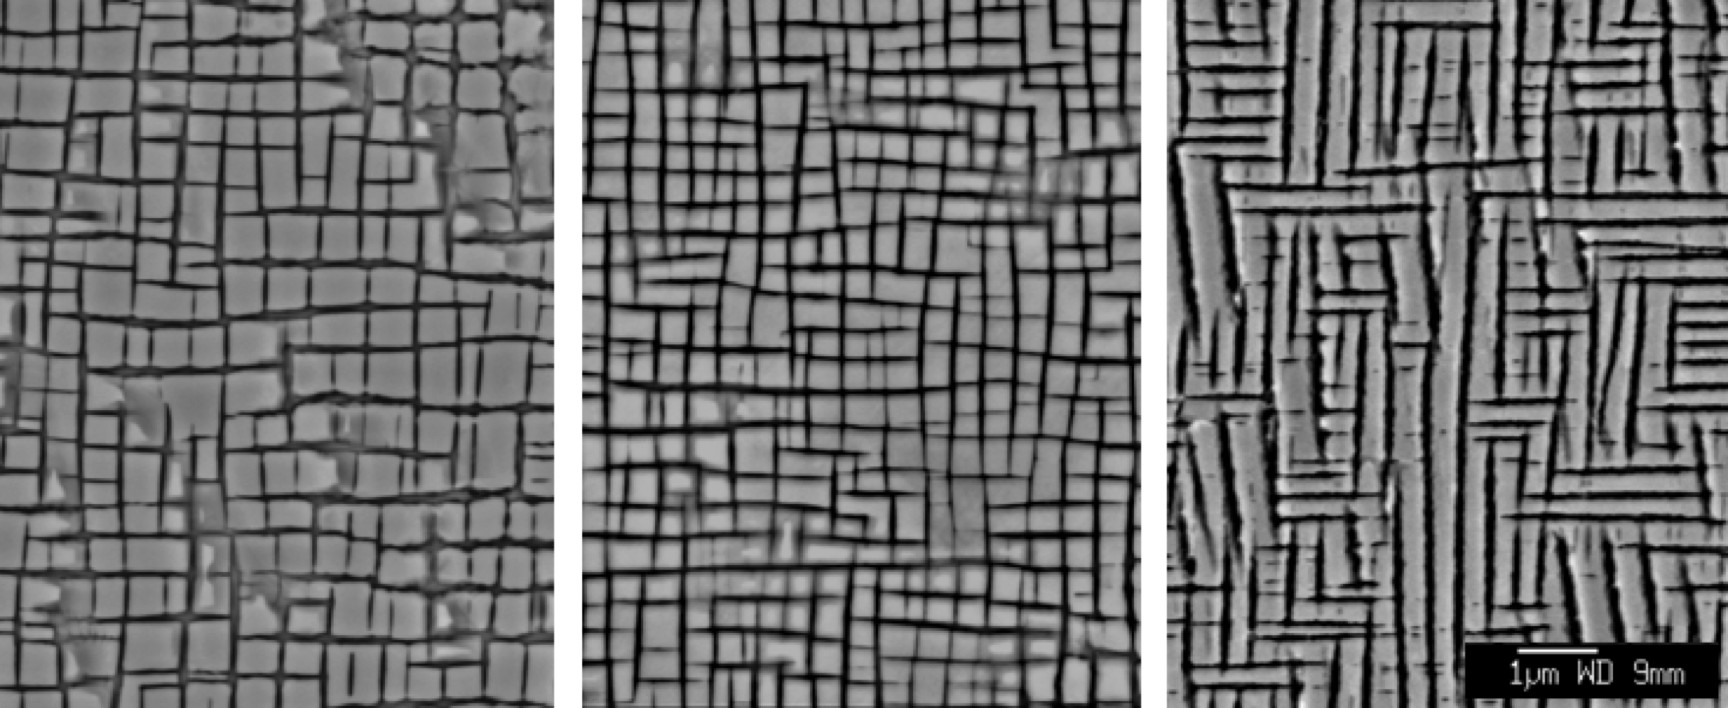
\includegraphics{LDSXAsAged}
\caption{LDSX--1, 6 and 8: as aged}\label{fig:LDSXAsAged}
\end{center}
\end{figure} 
%
\begin{figure}[hp]
\begin{center}
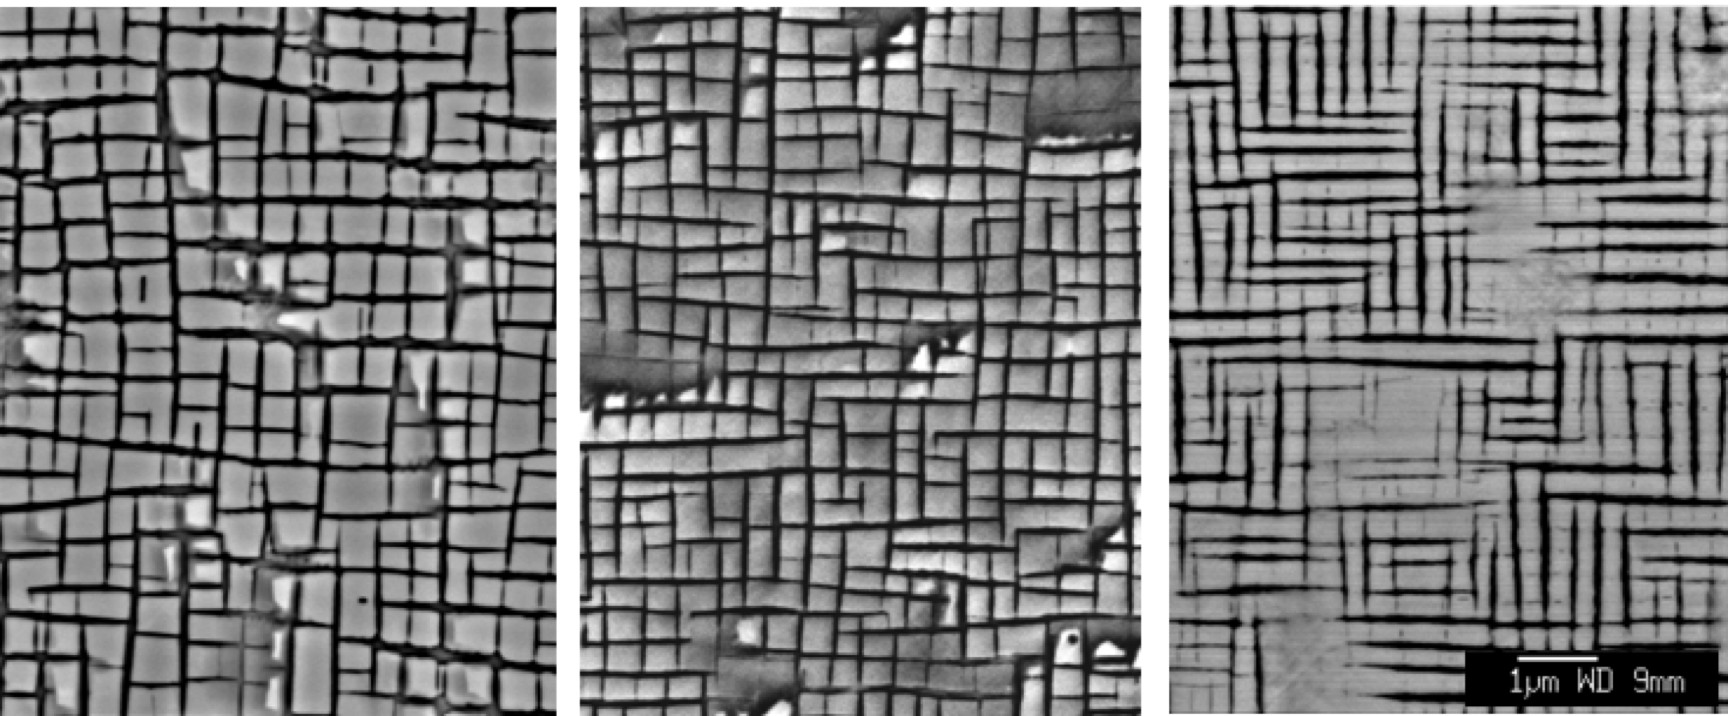
\includegraphics{LDSXInterrupted}
\caption{LDSX--1, 6 and 8: as interrupted crept }\label{fig:LDSXInterrupted}
\end{center}
\end{figure} 
%
\begin{figure}[hp]
\begin{center}
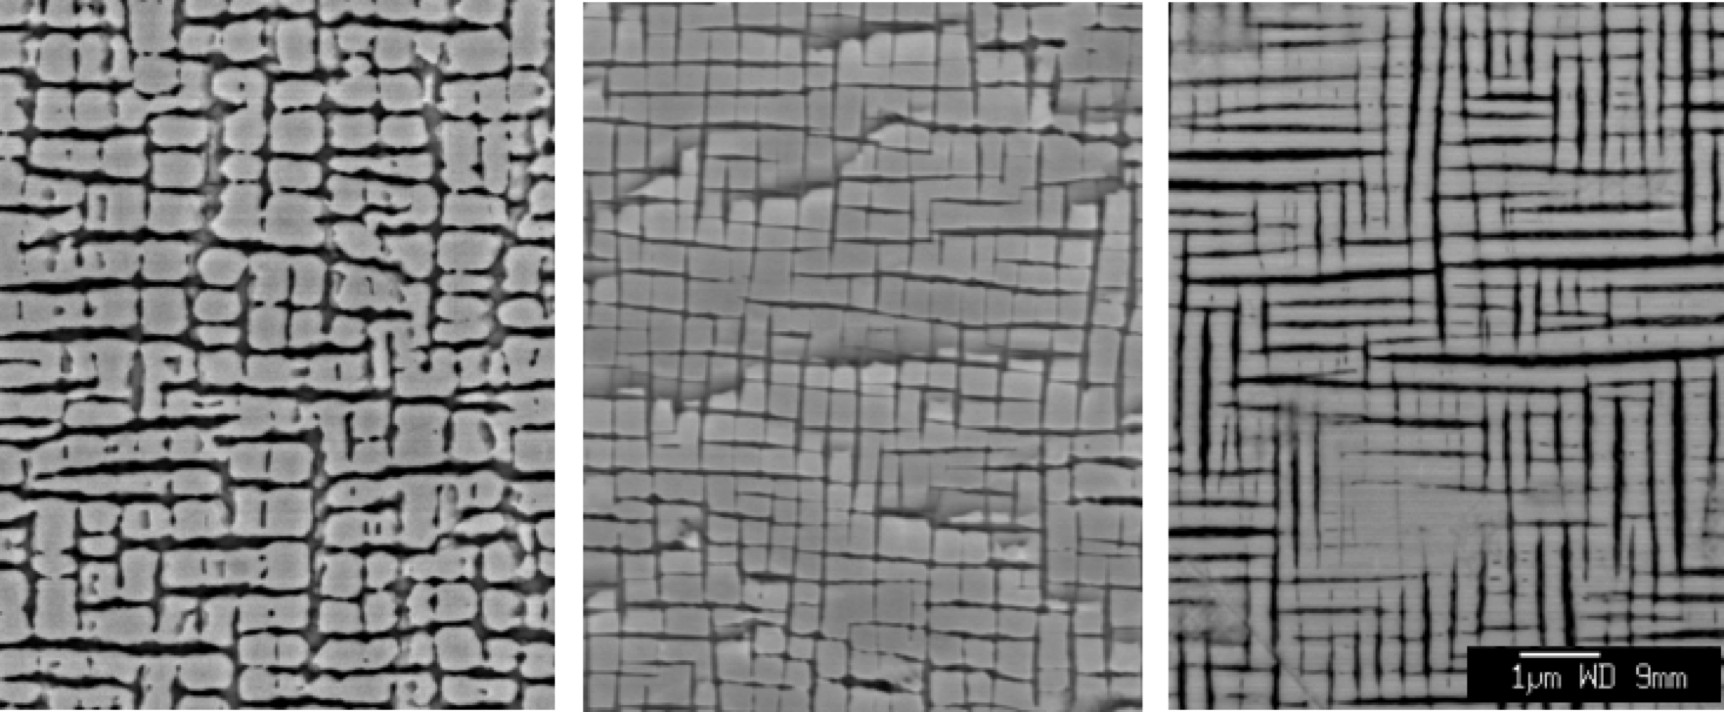
\includegraphics{LDSXInterrupted_10}
\caption{LDSX--1, 6 and 8: as interrupted crept + 10 hours at 950\celsius}\label{fig:LDSXInterrupted_10}
\end{center}
\end{figure} 
%
\begin{figure}[hp]
\begin{center}
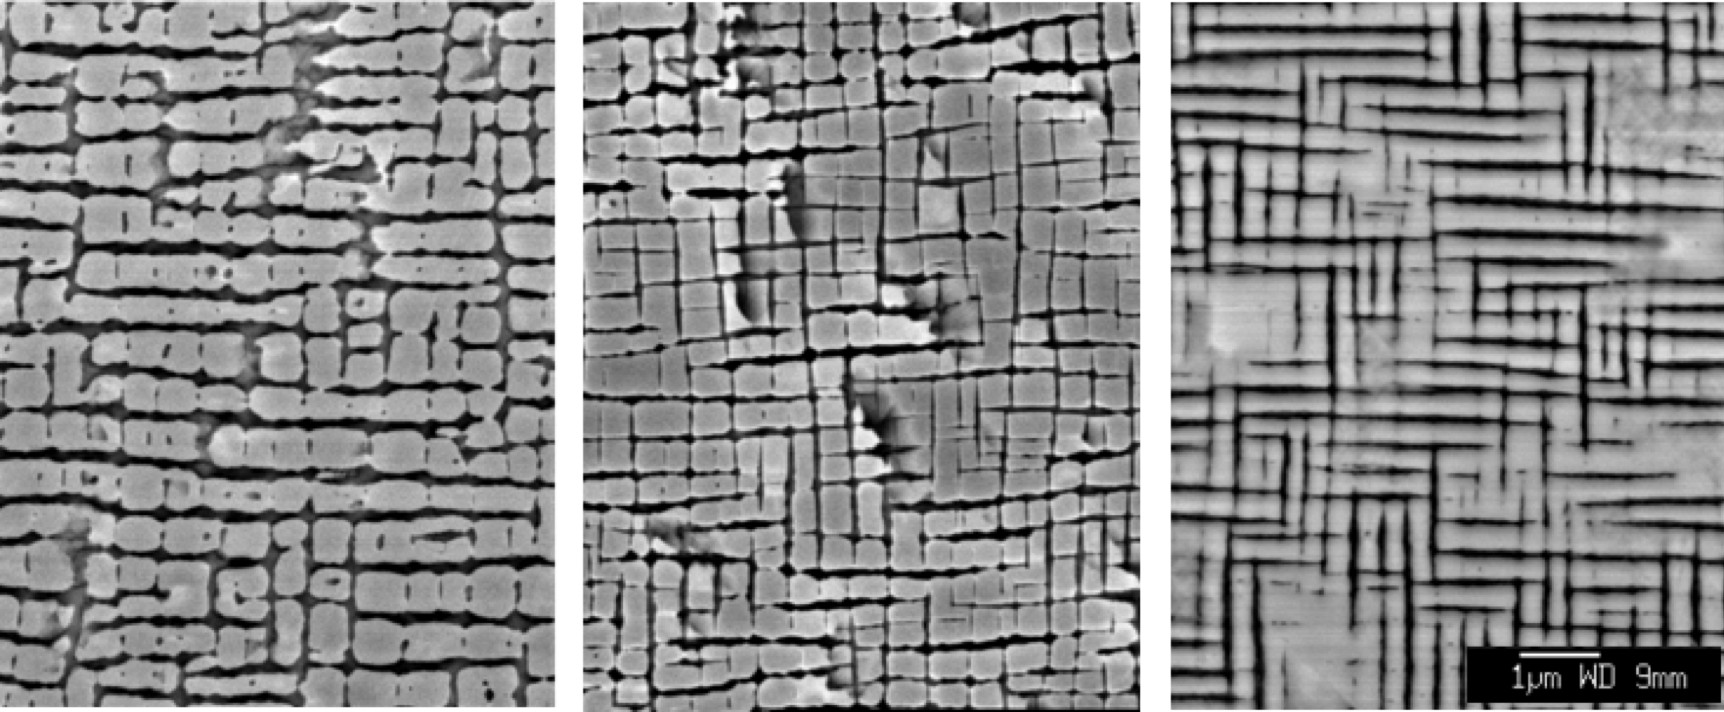
\includegraphics{LDSXInterrupted_50}
\caption{LDSX--1, 6 and 8: as interrupted crept + 50 hours at 950\celsius}\label{fig:LDSXInterrupted_50}
\end{center}
\end{figure} 
%
\begin{figure}[hp]
\begin{center}
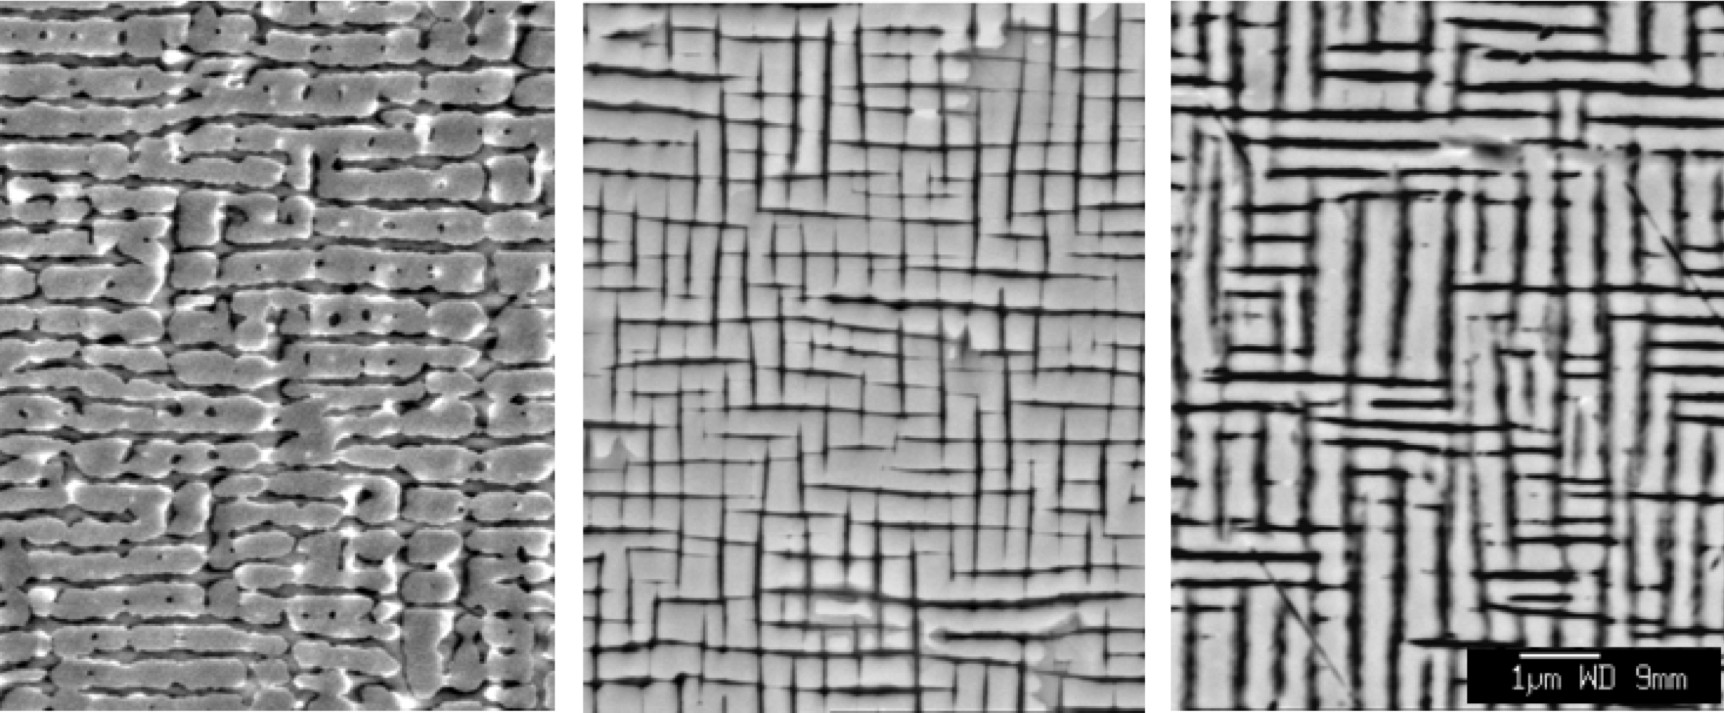
\includegraphics{LDSXInterrupted_200}
\caption{LDSX--1, 6 and 8: as interrupted crept + 200 hours at 950\celsius. }\label{fig:LDSXInterrupted_200}
\end{center}
\end{figure} 
%
\begin{figure}[hp]
\begin{center}
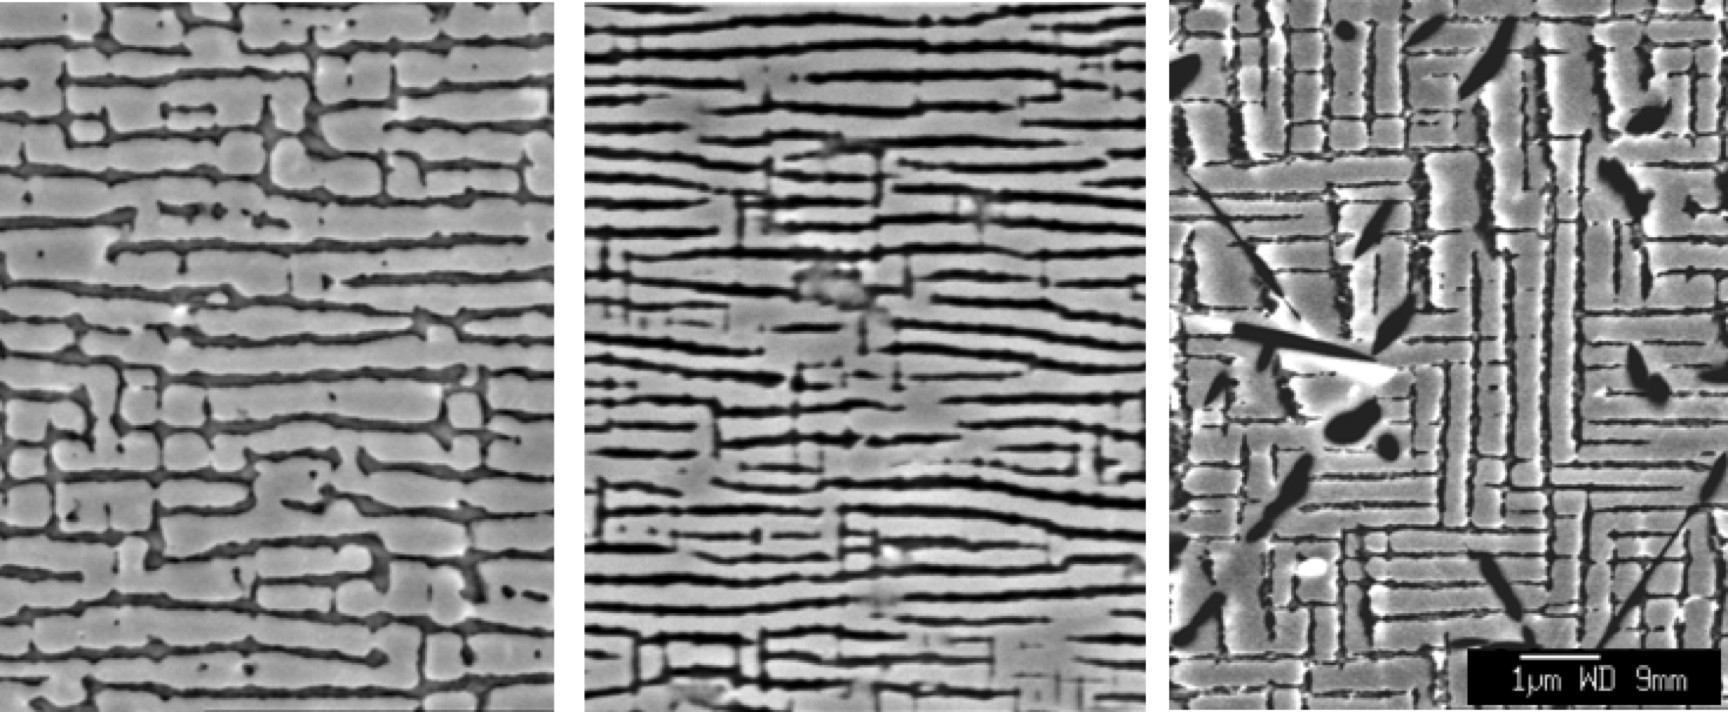
\includegraphics{LDSXInterrupted_500}
\caption{LDSX--1, 6 and 8: as interrupted crept + 500 hours at 950\celsius.}\label{fig:LDSXInterrupted_500}
\end{center}
\end{figure}
%
In LDSX--6, some TCP precipitation was seen in the dendrite core regions after 200 additional hours at 950\celsius\ (Figure \ref{fig:LDSXInterrupted_200}).  The volume fraction of precipitates is not substantial enough to adversely affect creep properties.  This is consistent with LDSX--6 having the longest creep life.  

Dislocations were observed in the $\gamma$ channels of the as heat treated LDSX--8 in TEM (Figure \ref{fig:LDSX8disloc}). They were unobservable in the as heat treated SEM sample (Figure \ref{fig:LDSXAsAged}) because the specimen was sectioned at an angle to the $\{001\}$ plane, which did not allow large portions of $\gamma$ channels to be observed.  The presence of dislocations prior to application of stress is quite unusual.  Dislocation networks became noticeable in the dendritic regions of the interrupted creep specimen after a subsequent thermal exposure of 10 hours (Figure \ref{fig:LDSXInterrupted_10}).  Their density increased with thermal exposure length.  Their presence indicates that the $\gamma$/$\gamma'$ interfaces have lost coherency by forming these stress-relieving networks (Figure \ref{fig:LDSX8disloc}).  

LDSX--8 is microstructurally unstable.  Rampant precipitation was observed after 200 hours at 950\celsius, and most dendritic regions contained substantial TCP precipitates (Figure \ref{fig:LDSXInterrupted_200}).  This extensive TCP precipitation is detrimental to creep properties, as it depletes the surrounding microstructure of strengthening elements.  The removal of these elements reduces the alloy's lattice misfit, but rafting was not halted nor reversed, as can be seen in the specimen that had been exposed for 500 hours at 950\celsius\ (Figure \ref{fig:LDSXInterrupted_500}). 

It is difficult to isolate the influence that lattice misfit has on creep from the influence of the extent of TCP precipitatation; these two factors have a very strong correlation, as can be seen in LDSX--8.  Lattice misfit becomes more negative upon the addition of select refractory elements; this also increases rafting and promotes TCP precipitation. 

The premature failure of LDSX--8 in creep will have to be attributed to both its highly rafted labyrinth structure and the extensive precipitation of TCPs.  Figure \ref{fig:LDSXCreep} shows time to \% strain for the three alloys.  LDSX--8 showed the poorest properties and took 60 hours to reach 1\% elongation.  The specimen with the closest thermal history available had been interrupted after 2 hours of primary creep at 950\celsius, and subjected to a further 50-hour thermal exposure (Figure \ref{fig:LDSXInterrupted_50}).  This specimen has a large population of dislocation networks.  The TCP precipitates visible are sparsely scattered, and are unlikely to adversely affect the mechanical properties of the alloy substantially.  From this, it can be said that the poorer performance of LDSX--8, as seen from its shorter time to 1\% elongation at 950\celsius\ when compared to LDSX--6, is exclusively due to its labyrinth structure.  The creep rupture time for LDSX--8 is even worse; it is half that of LDSX--6.  At this stage, TCP precipitation probably has a stronger negative influence than the labyrinth structure.

MacKay and Ebert state that the wider $\gamma$ channels resulting from rafting would adversely affect creep rates at 950\celsius.  Comparing the times to 0.5\% strain of the three alloys, strain rates increase with increasing misfit.  The alloy with the least propensity to raft, LDSX--1, has the longest time to 1\% strain.  This is consistent with the opinion of MacKay and Ebert ~\cite{mackay83}.  When we look at the times to 2\% strain, the strain rate of LDSX--6 between 0.5\% and 2\% is markedly slower than LDSX--1, as the time to 2\% strain is equal in both alloys.  These results suggest that wider $\gamma$ channels impact creep only to a small extent, and this impact is limited to initial creep strain.  These channels may allow the dislocations to travel a larger distance with ease, but once the dislocations encounter a $\gamma'$ precipitate, they are captured at the $\gamma$/$\gamma'$ interface, and cannot travel further.  In fact, we suggest that the $\gamma'$ precipitates in LDSX--6 may be stronger than those in LDSX--1 due to the higher content of refractory elements present, and they pose a larger resistance to precipitate cutting by dislocations, thereby improving creep resistance and allowing for LDSX--6 to display a longer time to creep rupture than LDSX--1.

An increase of misfit improves creep performance, but a misfit larger than the optimum level is is detrimental to creep. We do not see an adverse effect due to the extent of rafting; LDSX--6 rafts to a greater extent than LDSX--1, but has better creep properties.  A negative effect is only seen when the labyrinth structure is present. 

The diffusion coefficient of $\gamma$ is one magnitude higher than that of $\gamma'$, and allows the refractory elements to cluster together with more ease in the former, nucleating TCP precipitates ~\cite{reed06}.  This is why TCP precipitates are mostly located in the wider $\gamma$ channels where there are substantial dislocation networks.  These networks serve as fast diffusion paths for the slow-diffusing refractory atoms to agglomerate into TCP precipitates.  It is interesting to note that although LDSX--6 is less stable than LDSX--1 with respect to TCP precipitation, it is also stronger with the slowest creep at all strains above 2\% (Figure \ref{fig:LDSXCreep}).   

These results suggest there is an upper limit on the useful magnitude of the negative misfit and thus the concentration of refractory elements used to strengthen the $\gamma$-matrix at intermediate temperatures.  At lower temperatures, misfit appears beneficial for creep at 750\celsius.  But as the temperature rises, high misfit can cause spontaneous rafting to give a labyrinth structure.  This appears to be detrimental for creep at 950\celsius\ even before substantial TCP precipitation is observed.  This can be tested by producing a microstructure in LDSX--8 without the labyrinth rafting through a suitable heat treatment.
%
\begin{figure}[H]
\begin{center}
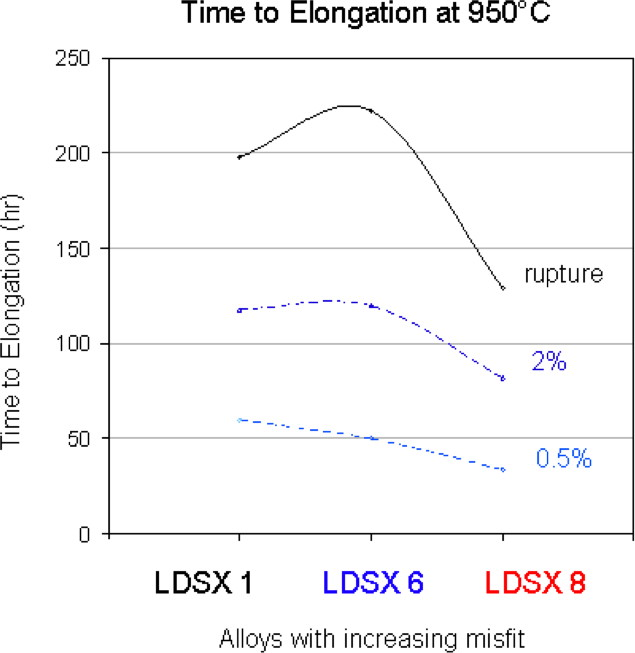
\includegraphics[width=9cm]{LDSXCreep}
\caption{Time to \% percent elongation of LDSX--1, 6 and 8 at 950\celsius/ 375\mega\pascal.}
\label{fig:LDSXCreep}
\end{center}
\end{figure}
%
\begin{figure}[H]
\begin{center}
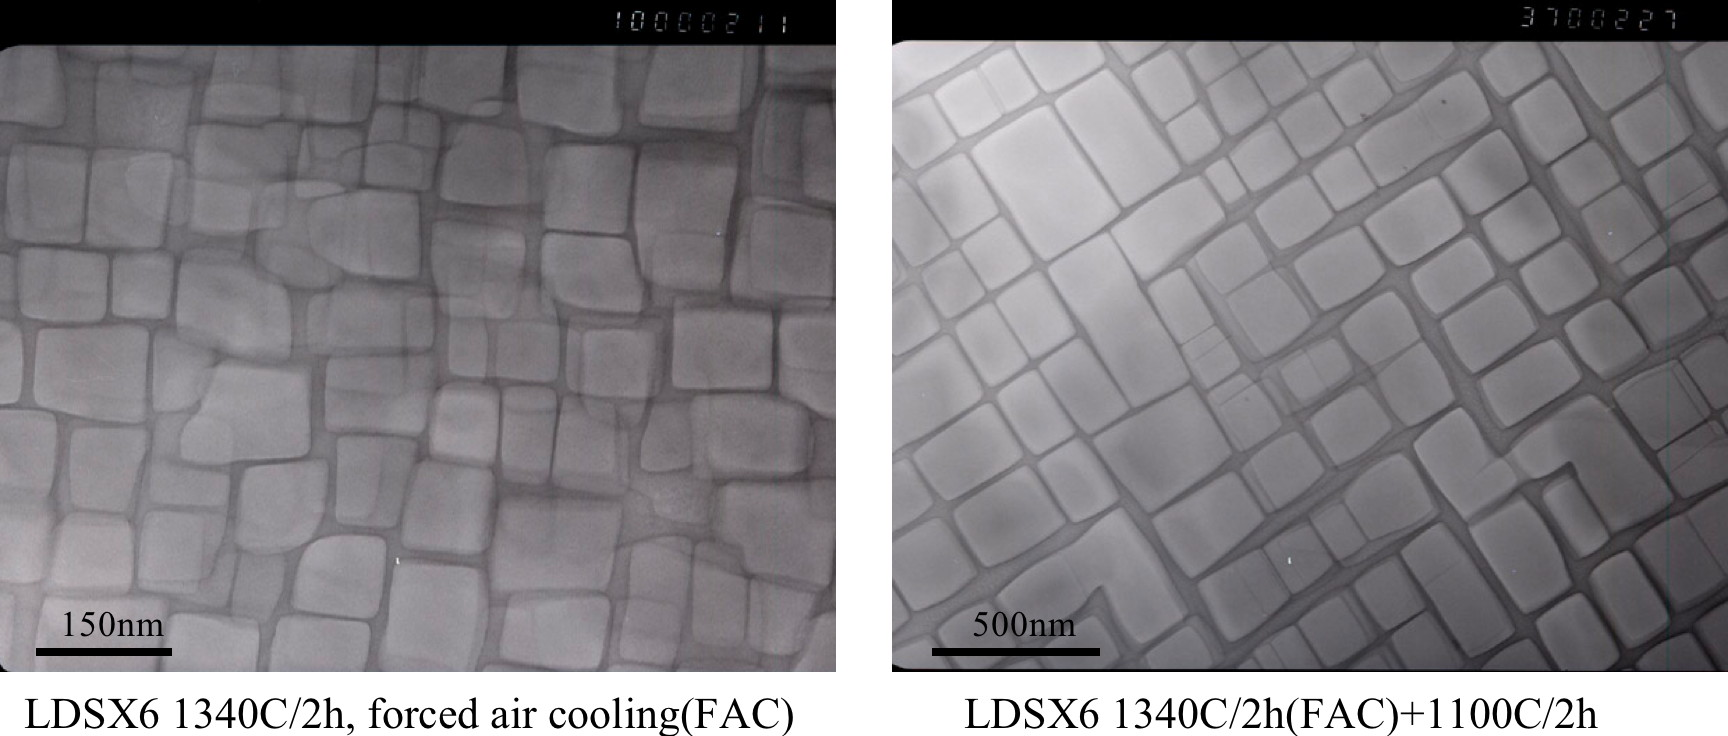
\includegraphics{LDSX6HT}
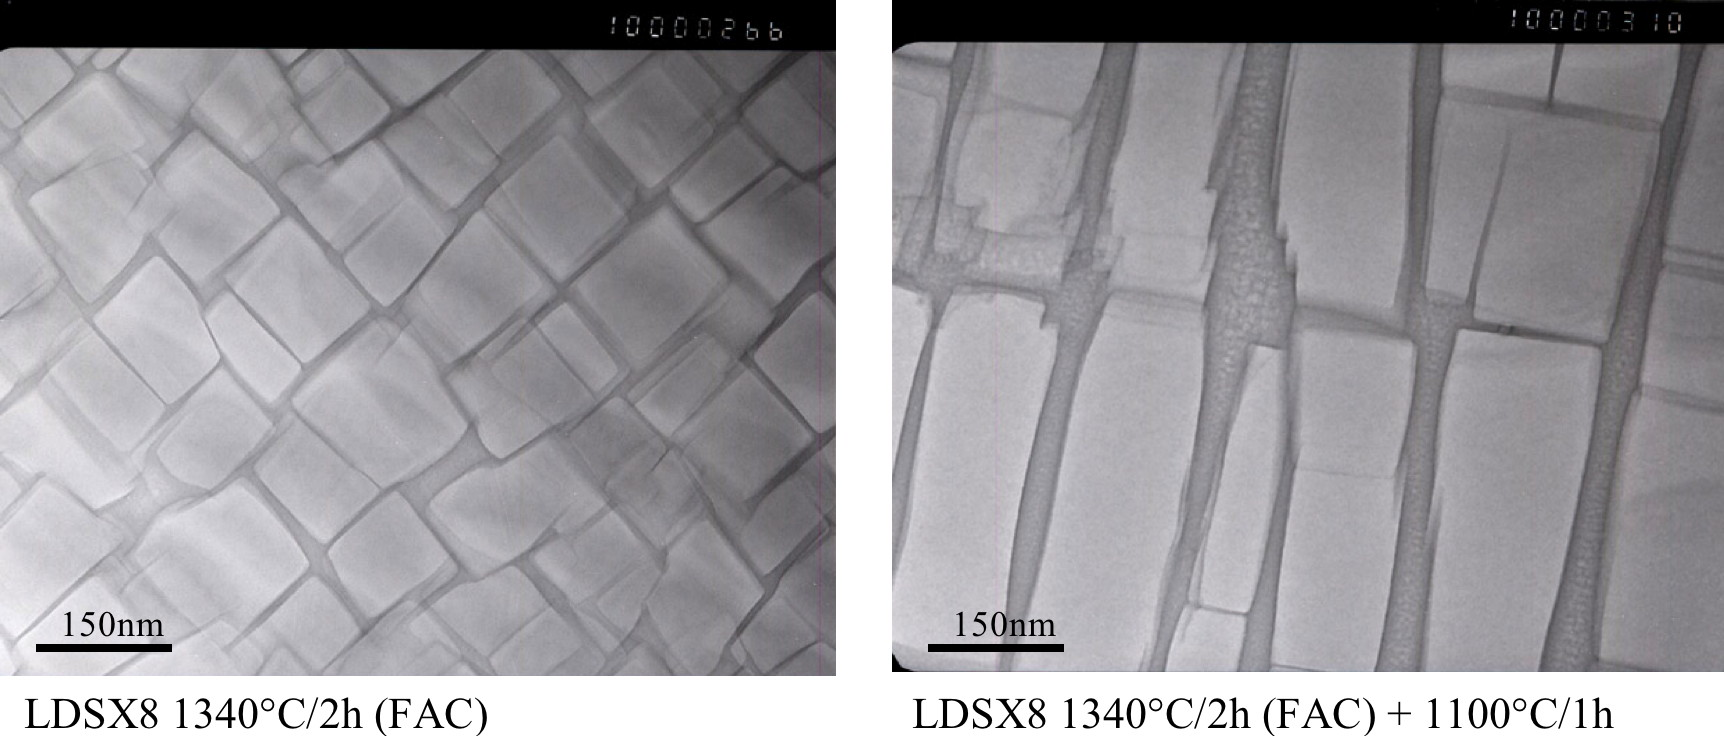
\includegraphics{LDSX8HT}
\caption{TEM micrographs of LDSX--6 and 8 after various heat treatments.}
\label{fig:LDSXHT}
\end{center}
\end{figure}
\vspace{-8mm}
%
Typically, a nickel-base superalloy that has been homogenised has to undergo an ageing treatment to achieve a uniform distribution of cubiodal $\gamma'$ precipitates.  This ageing treatment is performed at 1100\celsius\ for a few hours, as this is the temperature required for the diffusion step of the application of low-cost platinum-aluminised bond coats used as protection against high temperature corrosion and oxidation ~\cite{reed06}.  As seen in Figure \ref{fig:LDSXHT}, the $\gamma'$ precipitates of LDSX--6, become more cuboidal and orderly after 2 hours at 1100\celsius .  

Figure \ref{fig:LDSXHT} shows the microstructures of LDSX--6 and 8 after an additional solution heat treat of 2 hours at 1340\celsius\ followed by an air quench.  This process produces a finer $\gamma'$ size than conventional cool in a commercial furnace.  In the case of the highly misfitting LDSX--8, precipitate coalescence occurs after 1 hour at 1100\celsius, which is disadvantageous for low and intermediate temperature creep.  The as-homogenised LDSX--8 specimen that underwent an additional 1340\celsius\ for 2 hours seems to have a sufficiently optimised microstructure; the $\gamma'$ precipitates are cubiodal.  If the labyrinth structure seen in the as-aged specimen is detrimental to the creep properties of LDSX--8, the as-homogenised specimen should out-perform the as-aged specimen in creep.  A creep test at 950\celsius/ 375\mega\pascal\ will be conducted on this as-homogenised sample and compared to the creep results of the as-aged specimen.  This will indicate the extent of which labyrinth rafting is causing the poor creep properties.

\subsection{Measurement of Lattice Misfit}

Two-dimensional and three-dimensional plots (Figure \ref{fig:3Dplot}) of intensity in reciprocal space were obtained at the ESRF. There are two $\gamma$ peaks due to the different lattice parameters of the constrained $\gamma$ in the vertical channels and the unconstrained $\gamma$ in the horizontal channels. The peaks from $\gamma'$ and the constrained $\gamma$ were fitted, and theirlattice parameters were used to calculate the lattice misfits using Equation \eqref{eq:misfit}. The calculated misfit values (Table \ref{tab:misfitesrf}) are higher than the predicted values (Table \ref{tab:misfitjmatpro}). 
 
\begin{figure}[H]
\begin{center}
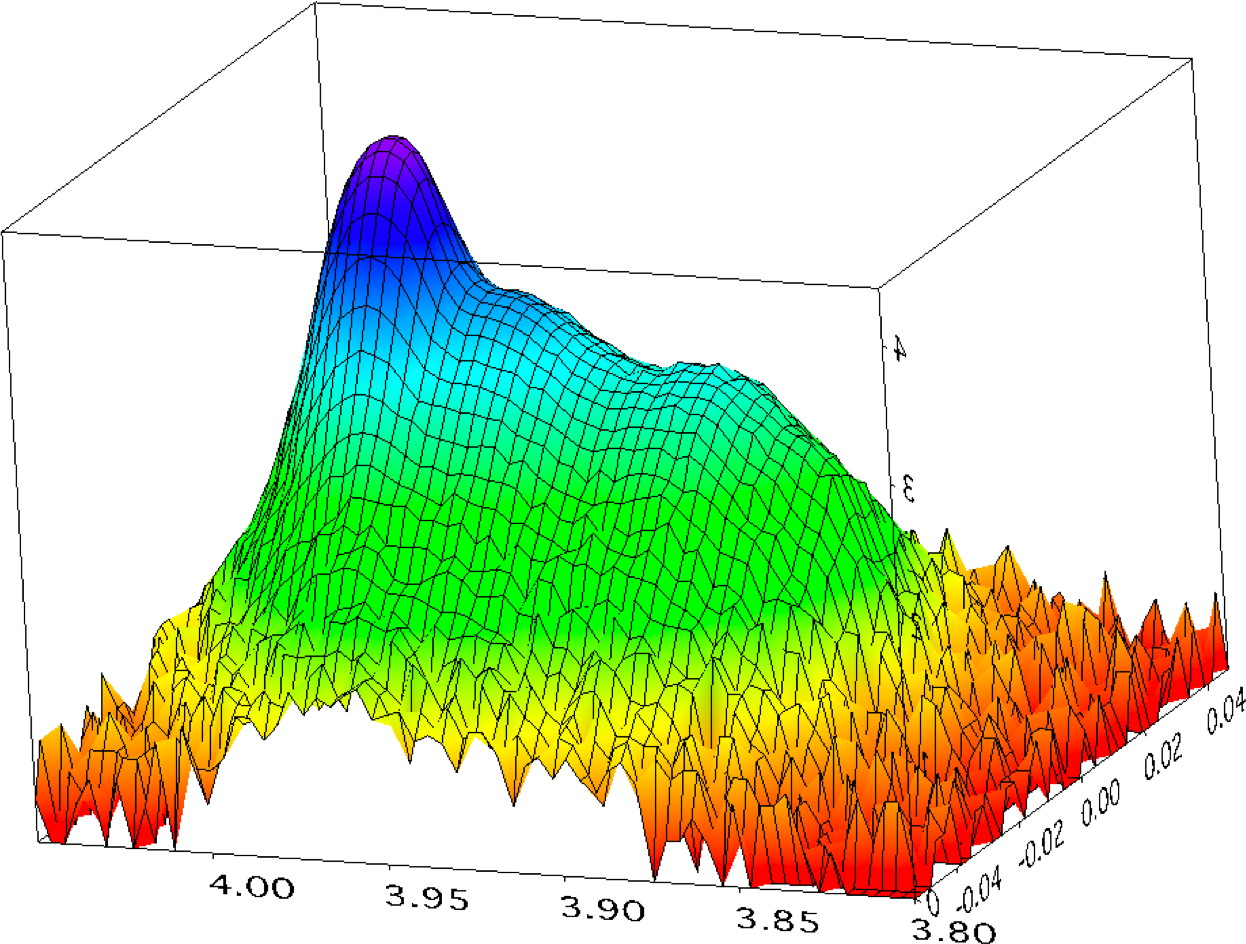
\includegraphics{3Dplot}
\caption{3D plot of LDSX--8 as HT}\label{fig:3Dplot}
\end{center}
\end{figure}

 
%
\begin{table}[H]
\begin{center}
\begin{tabular}{l c c c c} 
\hline
\hline
Alloy & 	Phase    &	Reciprocal lattice distance   &Lattice distance &	Misfit 	\\
\hline
\multirow{2}{*}{LDSX--1}&	$\gamma$ &	3.96944					&3.62029	&	\multirow{2}{*}	{-0.77\%}	\\
	 &	$\gamma'$&	4.00004					&3.59259	&				\\
\multirow{2}{*}{LDSX--6}&	$\gamma$ &	3.96443					&3.62486	&	\multirow{2}{*}	{-0.85\%}	\\
 	 &	$\gamma'$&	3.99827					&3.59418	&				\\
\multirow{2}{*}{LDSX--8}&	$\gamma$ &	3.96783					&3.62176	&	\multirow{2}{*}	{-0.78\%}	\\
	 &	$\gamma'$&	3.99896					&3.59356	&				\\
\hline
\hline
\end{tabular}
\end{center}
\caption{Lattice misfit values of LDSX--1, 6 and 8, obtained at the ESRF. }
\label{tab:misfitesrf}
\end{table}


\begin{table}[H]
\begin{center}
\begin{tabular}{l c c } 
\hline
\hline
Alloy&	Temp (\celsius) &	Misfit (\%)\\
\hline
&	25	&-0.11\\
CMSX-4	&900	&-0.25\\
	&1100&-0.25\\
	\hline
&	25	&-0.22\\
LDSX--1	&900	&-0.30\\
	&1100&	-0.30\\
	\hline
&	25	&-0.31\\
LDSX--2	&900	&-0.41\\
	&1100&	-0.41\\
	\hline
&	25&	-0.36\\
LDSX--3	&900&	-0.47\\
	&1100&	-0.44\\
	\hline
&	25	&-0.22\\
LDSX--4	&900	&-0.30\\
	&1100&	-0.30\\\hline
&	25&	-0.25\\
LDSX--5	&900	&-0.33\\
	&1100&	-0.33\\
	\hline
&	25&	-0.28\\
LDSX--6	&900	&-0.36\\
	&1100&	-0.35\\
	\hline
&	25&	-0.39\\
LDSX--7	&900	&-0.44\\
	&1100&	-0.44\\
	\hline
&	25&	-0.39\\
LDSX--8	&	900&	-0.47\\
	&	1100&	-0.49\\
\hline
\hline
\end{tabular}
\end{center}
\caption{Lattice misfit values of LDSX--1, 6 and 8, predicted by JMatPro$^{\copyright}$. }
\label{tab:misfitjmatpro}
\end{table}